\section{Supplementary Information/Appendix}

\subsection{Site Intercomparison of Baring Head and Cape Grim}


\begin{figure}[htp]
    \centering
    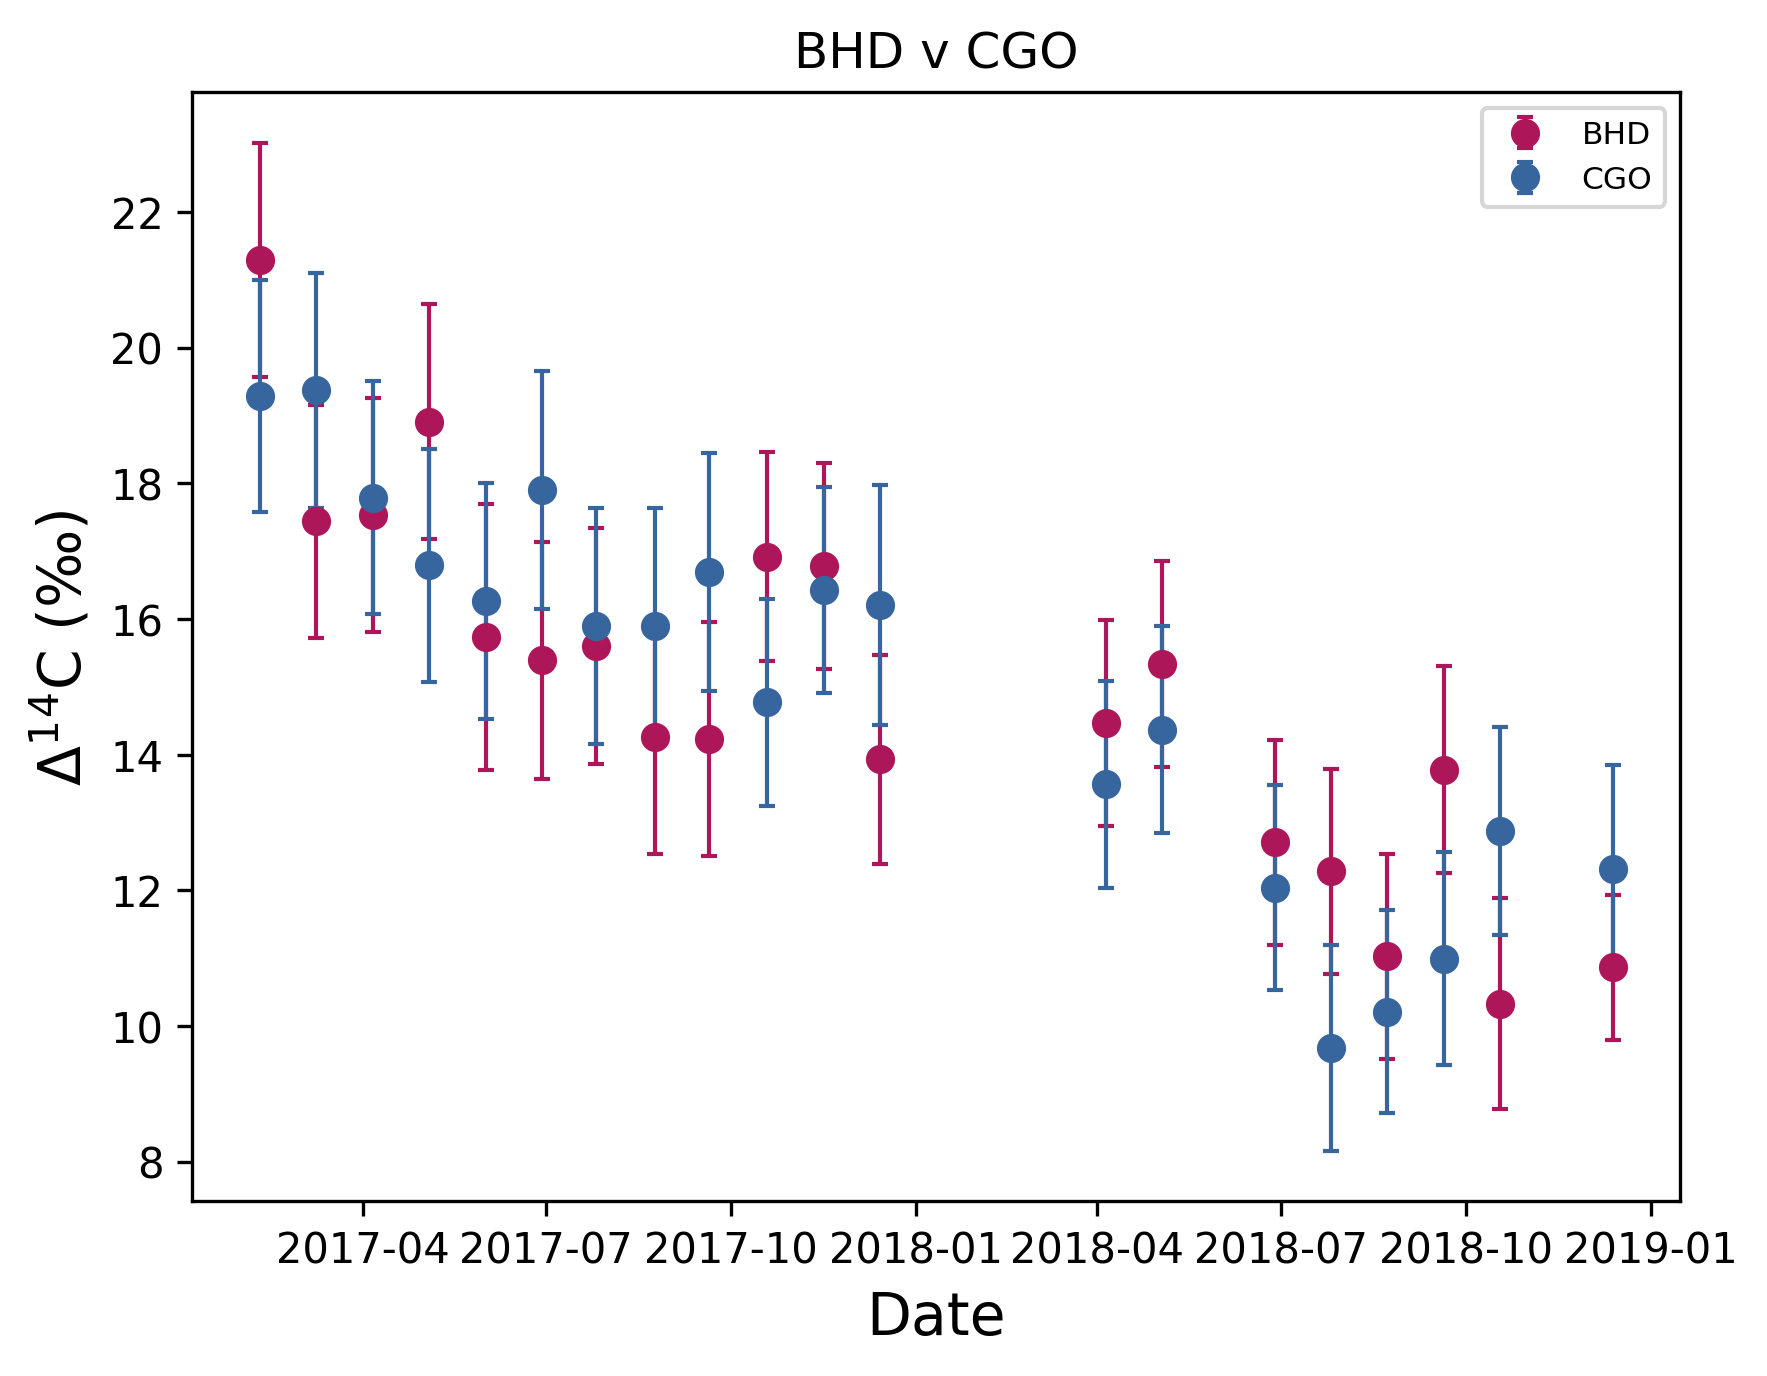
\includegraphics[width=12cm]{plots/Site_intercomparison.png}
    \caption{Intercomparison of ${\Delta^{14}CO_{2}}$ measurements  at Cape Grim, Tasmania (CGO), and Baring Head, New Zealand (BHD) collected by NIWA and measured at Rafter Radiocarbon Laboratory. Dates represent the middle of the sampling period, which differ no more than one day between sites. These data show that during the time in which data are available, no measureable difference is found between the two sites. This provides some evidence that the two sites may be considered equivalent for this intercomparability study.}
    \label{fig:bhdvcgo}
\end{figure}


The following process occurs during each iteration for both BHD and CGO data: 
\begin{itemize}
	\item For each x-value, the y-value is  randomly re-assigned, weighted about its normal distribution (1-${\sigma}$ error). 
	\item This randomized time-series is smoothed/trended with CCGCRV algorithm 
	\item The generated data (in 348 equal steps from 1987 to 2016) is appended to a growing dataframe of smoothed/trended data.
\end{itemize}
When the loop is complete, the mean and standard deviation of y each 348 x-values is calculated for BHD and CGO. These computed values are used to assess the intercomparability of BHD and CGO, and thus, Rafter Radiocarbon Lab and Heidelberg University over time. This Monte-Carlo simulation is shown on a small scale in Figure \ref{fig:montecarloexplained}. Statistics are then computed for each of the four time-intervals described above. 

\begin{figure}[htp]
    \centering
    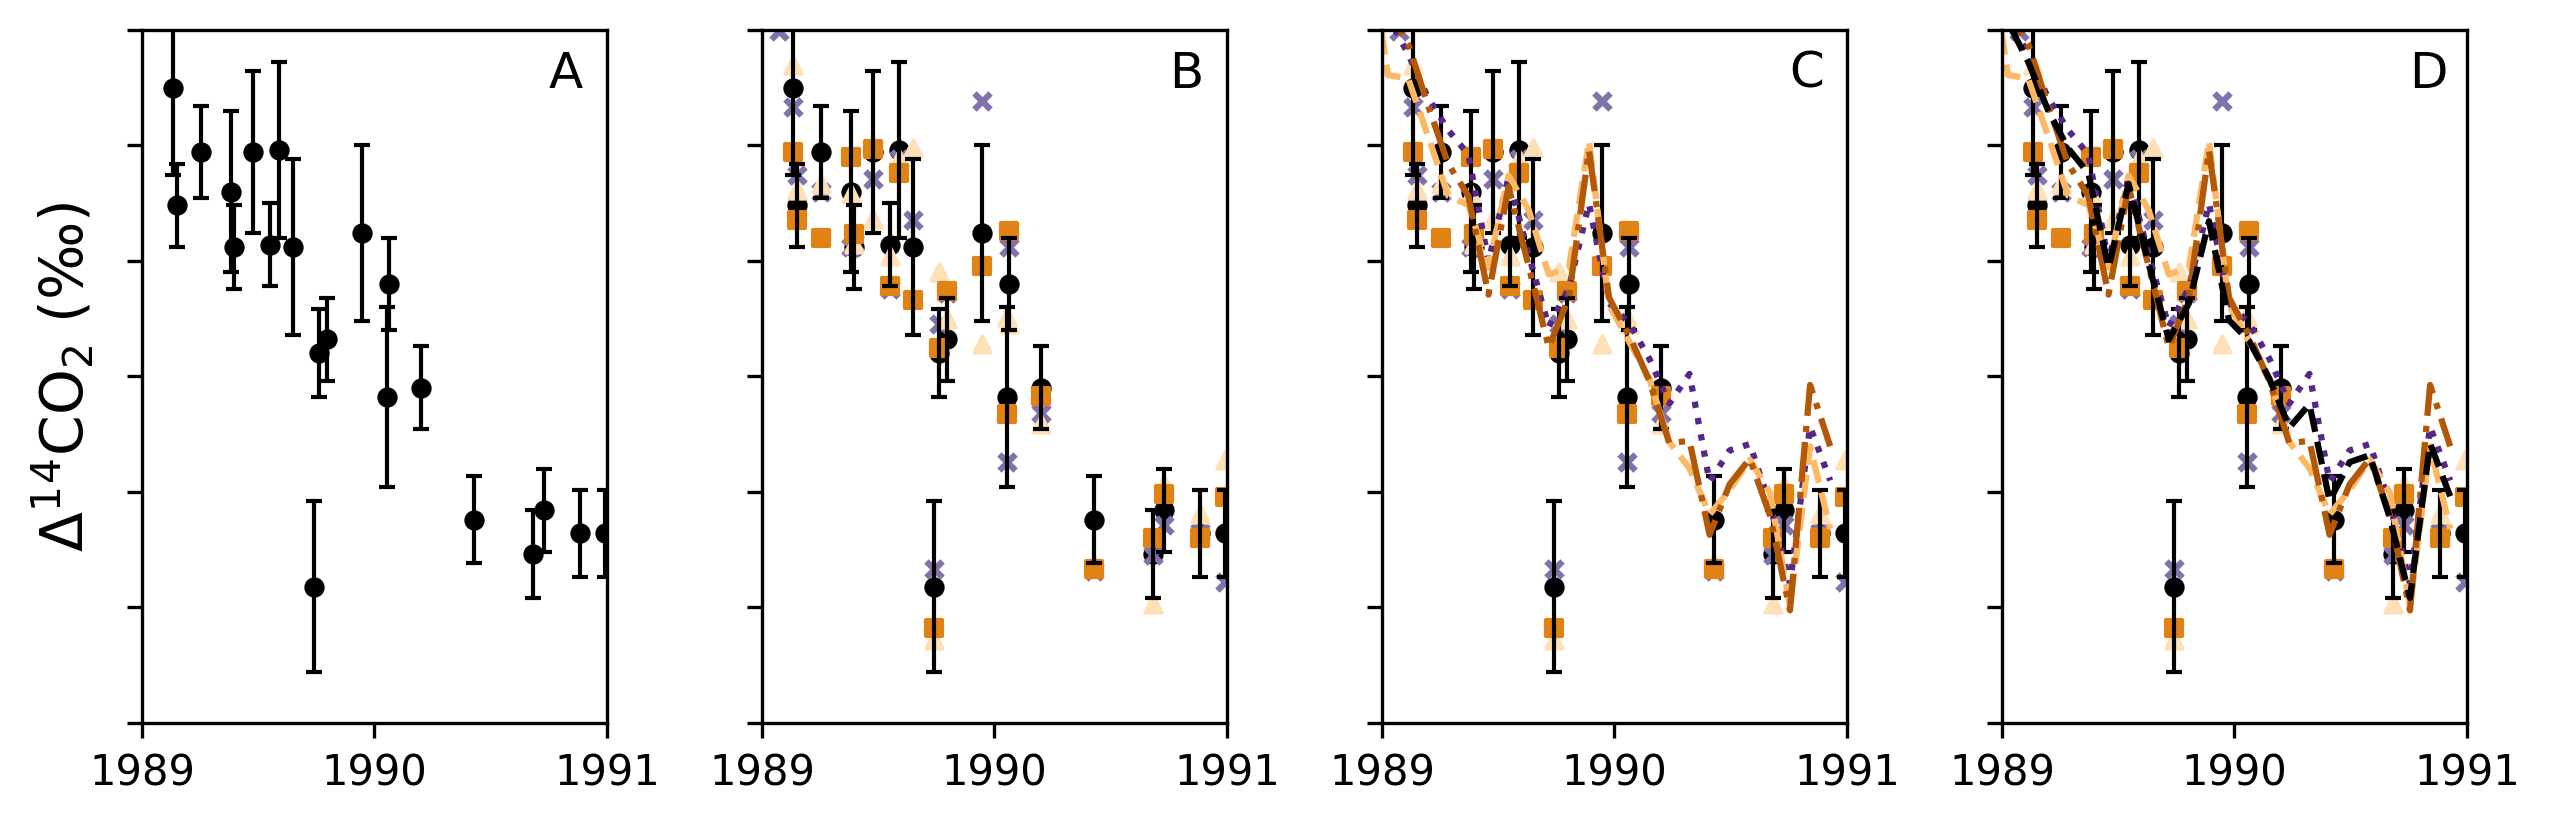
\includegraphics[width=\textwidth]{plots/DEV_FirstDraft_figureS1.png}
    \caption{Visualization of the Monte Carlo simulation to generate an uncertainty estimate about the CCGCRV curve smoothing algorithm.}
    \label{fig:montecarloexplained}
\end{figure}